\title{Git Assistant}
\author{Ali AlShami}


%Main body starts
\section{Introduction}
I am working through my first year as a provisional Ph.D. student in the Security program, so I have taken the 
classes required to complete my provisional status. I am taking the last of the four required courses this semester and 
will be moved into a full Ph.D. Student status. However, Dr. Xu already has me doing a couple of introductory
 research projects as I am new to the interworkings of researchers outside of compliance.
  I seek to gain valuable insight into the generalizations on how to properly research so that as I become a researcher,
   I can build a research style of my own. I do not have a foundation in research, so I want to build a solid foundation to grow. 
   Having worked in the technology field for the past ten years, I have found two rules always to be true, "you don't know what you don't know,"
    and those who do not seek knowledge will not gain understanding. I want to be a cybersecurity expert, which means I have a lot of knowledge 
    that I don't know, and a lot that I do know; however, I will never be stagnant in my pursuit of knowledge. This is why research is 
very appealing to me because now I am seeking an ability that no one might know or building upon known knowledge but has evolved.  

\begin{figure}[hbt!]
    \centering
    \includegraphics[width=5cm]{Gwartney.jpg}
    \caption{ }
    \label{fig:Remove}
\end{figure}

\section{Related code}

\url{https://github.com/harrisasadb/Clustering-Cyber-Security-Metrics-of-Companies}

\begin{figure}[ht]
\centering
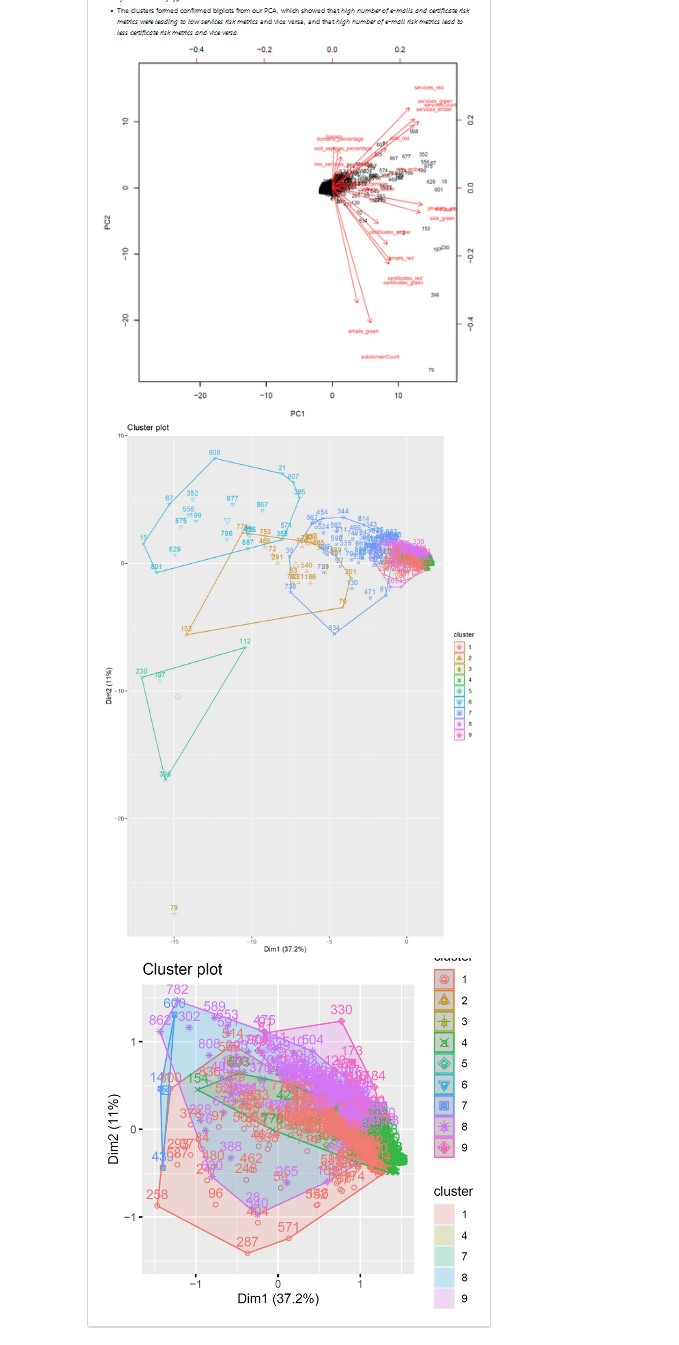
\includegraphics[angle=0,width=.7\linewidth]{GitAssignmentClustering.jpg}
\caption{Examples of Clustering Based on R code} 
\label{fig:view}
\end{figure}
\bigskip


\begin{figure}[ht]
\centering
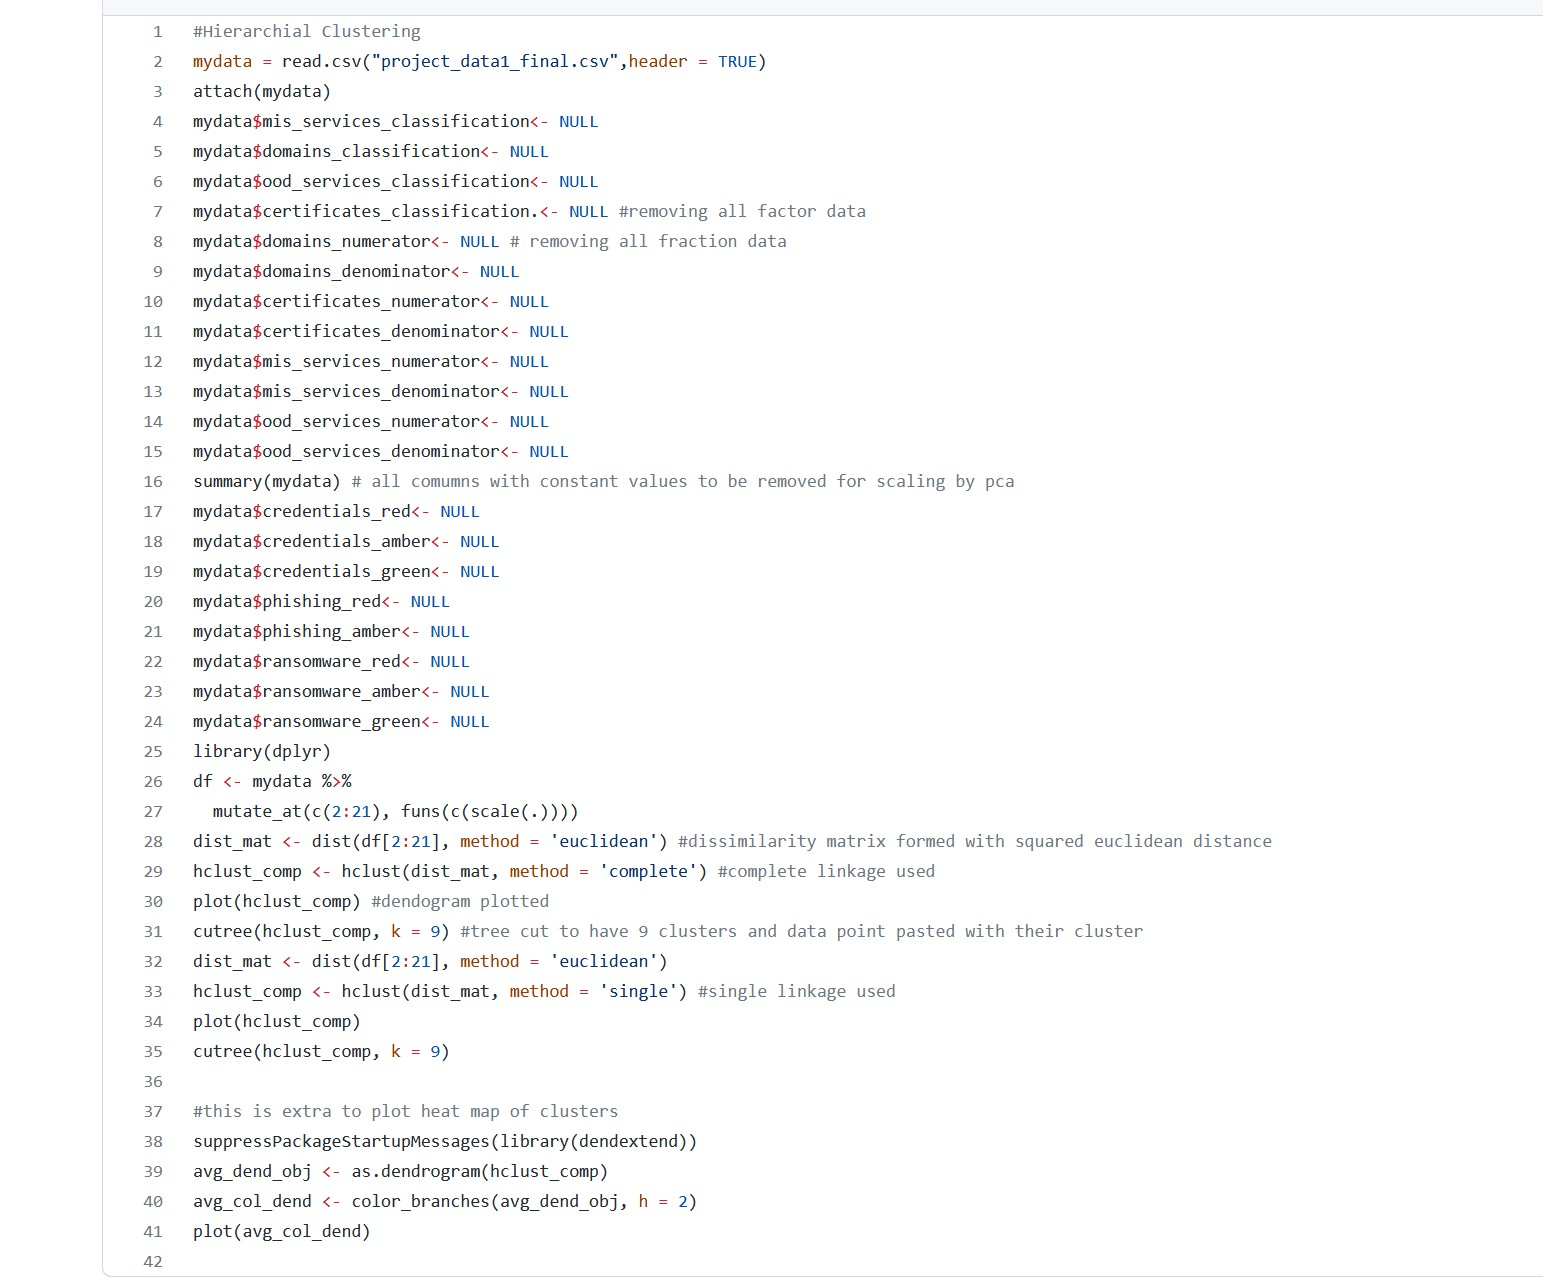
\includegraphics[angle=0,width=.7\linewidth]{R-Code-Her.jpg}
\caption{Hierarchical Clustering.R} 
\label{fig:view}
\end{figure}
\bigskip

\section{Question}
Which area of security are you focusing on?


\end{document}
